\section{Experiment}

\subsection{Experiment Settings}\label{exp:setting}

\textbf{RL Training}
We conducted training experiments using DAPO~\citep{dapo} and GRPO~\citep{grpo} on two prominent mathematical reasoning datasets: GSM8K~\citep{cobbe2021training} and BigMath~\citep{albalak2025big}. GSM8K comprises 7,500 samples with a generation number of 8, while BigMath includes 122,000 samples with a generation number of 16. Both datasets feature problems of medium to high difficulty, spanning levels 3 to 5. For GSM8K, we trained 3B and 7B models, whereas for BigMath, we trained 7B, 14B, and 32B models. Specifically, the 7B and 14B models were trained on problems ranging from levels 3 to 5, while the 32B model was exclusively trained on the more challenging level 4–5 problems. Training checkpoints were evaluated between 500 and 1000 steps. To account for the sensitivity of $Z_{noise}$ perturbation, we set its range from 5e-2 to 5e-4 for dynamic noise estimation. In the main experiments, the LoRA rank is fixed at 32. The speedup tests are performed on a single H100 GPU, while the final evaluated model is trained using 8 H100 GPUs to ensure experimental efficiency on such large-scale data. Detailed hyperparameters and deployment of QeRL are provided in Appendix~\ref{ap:hyper} and Appendix~\ref{ap:pseudocode}.

\textbf{Backbone Models}
We conduct experiments on Qwen2.5~\citep{team2024qwen2} series, using basic without any mathematic data fine-tuning. For weight-only quantization, we applied AWQ~\citep{lin2024awq} to MXFP4 and NVFP4 formats. The calibration dataset included 256 sequences, each 2048 tokens long, sampled from OpenThoughts-114k~\citep{guha2025openthoughts}. Weight-only formats also support inference acceleration on NVIDIA-H100 GPUs with the Marlin kernel~\citep{frantar2024marlin}. For NF4 quantization, we used the default configuration~\citep{qlora}.

\textbf{Evaluation Benchmarks and Metrics}
We focus on several widely used mathematical reasoning benchmarks, including GSM8K~\citep{cobbe2021training}, MATH500~\citep{lightman2023let}, AIME 2024/2025~\citep{li2024numinamath}, and AMC 23~\citep{li2024numinamath}, for evaluation. During inference, we use a temperature of 0.6, completion length of 4096, and top-p sampling with $p = 0.95$. Each data set is evaluated multiple times, and we report primarily the average accuracy of one sample (Pass@1).

\begin{table}[!t]
\vspace{-0.1in}
\centering
% First table (Qwen2.5-3B)
\begin{minipage}{0.48\textwidth} % 每个表格占据大约三分之一的文本宽度
\centering
\small % 调整字体大小
\caption*{(a) Performance of Qwen2.5-3B-Instruct.}
\vspace{-0.1in}
\begin{tabular}{lccl}
\toprule
\textbf{Model}      & \textbf{W\#} & \textbf{Training} &\textbf{GSM8K} \\ \midrule
\multirow{10}{*}{\makecell{Qwen2.5-3B \\-Instruct}} 
& BF16  & & 61.2 \\
\cdashline{2-4}
& NF4   & - &$57.5_{\textcolor{hangrey}{-3.7}}$ \\
& MXFP4  & - &$59.8_{\textcolor{hangrey}{-1.4}}$ \\
& NVFP4  & - &$59.4_{\textcolor{hangrey}{-1.8}}$\\ 
\cline{2-4}
&BF16 &Full&$84.4_{\textcolor{hanred}{+23.2}}$ \\
&BF16&LoRA&$76.1_{\textcolor{hanred}{+14.9}}$ \\
\cdashline{2-4}
&NF4&LoRA&$76.1_{\textcolor{hanred}{+14.9}}$ \\
&MXFP4&LoRA&$73.4_{\textcolor{hanred}{+12.2}}$ \\
&\cellcolor{hangrey!40}NVFP4&\cellcolor{hangrey!40}LoRA&\cellcolor{hangrey!40}$83.3_{\textcolor{hanred}{+22.2}}$ \\
&\cellcolor{hangrey!40}\textbf{}&\cellcolor{hangrey!40}\textbf{+AQN}&\cellcolor{hangrey!40}${83.7}_{\textcolor{hanred}{+22.6}}$ \\
\bottomrule
\end{tabular}
\end{minipage}% <-- 注意这里没有空行
\hfill % 在表格之间添加水平弹性空间
% Second table (Qwen2.5-7B)
\begin{minipage}{0.48\textwidth}
\centering
\small % 调整字体大小
\caption*{(b) Performance of Qwen2.5-7B-Instruct.}
\vspace{-0.1in}
\begin{tabular}{lccl}
\toprule
\textbf{Model}      & \textbf{W\#} & \textbf{Training} &\textbf{GSM8K} \\ \midrule
\multirow{10}{*}{\makecell{Qwen2.5-7B \\-Instruct}} 
& BF16  & - & 76.3 \\
\cdashline{2-4}
& NF4   & - &$70.5_{\textcolor{hangrey}{-5.8}}$ \\
& MXFP4  & - &$71.3_{\textcolor{hangrey}{-5.0}}$ \\
& NVFP4  & - &$73.4_{\textcolor{hangrey}{-2.9}}$\\ 
\cline{2-4}
&BF16 &Full&$91.2_{\textcolor{hanred}{+14.9}}$ \\
&BF16&LoRA&$88.1_{\textcolor{hanred}{+11.8}}$ \\
\cdashline{2-4}
&NF4&LoRA&$85.0_{\textcolor{hanred}{+8.7}}$ \\
&MXFP4&LoRA&$86.4_{\textcolor{hanred}{+10.1}}$ \\
&\cellcolor{hangrey!40}NVFP4&\cellcolor{hangrey!40}LoRA&\cellcolor{hangrey!40}$88.5_{\textcolor{hanred}{+12.2}}$ \\
&\cellcolor{hangrey!40}\textbf{}&\cellcolor{hangrey!40}\textbf{+AQN}&\cellcolor{hangrey!40}${90.8}_{\textcolor{hanred}{+13.5}}$ \\
\bottomrule
\end{tabular}
\end{minipage}% <-- 注意这里没有空行
%\vspace{-0.1in}
\caption{Qwen2.5 Performance on GSM8K. GRPO algorithm is used to train 3B and 7B models on GSM8K dataset, while ``Full'' denotes the full-parameter training and ``W\#'' represents the bit-width and data format of weight. \textcolor{hanred}{+} and \textcolor{hangrey}{-} are compared with original bfloat-16 (BF16) models.}
\label{tab:gsm8k}

\end{table}



\begin{table}[!t]
\vspace{-0.1in}
\centering
\resizebox{\columnwidth}{!}{
\begin{tabular}{lcclllll}
\toprule
\textbf{Model}      & \textbf{W\#} & \textbf{Training} &\textbf{MATH 500} &\textbf{AIME 24}&\textbf{AIME 25}&\textbf{AMC 23}&\textbf{Average}$\uparrow$\\ \midrule
\multirow{6}{*}{\makecell{7B}} 
& BF16  & - & 74.8&9.2&6.6&25.0&28.9 \\
% \cdashline{2-7}
% & NF4   &  &$70.5_{\textcolor{hangrey}{-5.8}}$ \\
% & MXFP4  & &$68.6_{\textcolor{hangrey}{-6.2}}$&$8.1_{\textcolor{hangrey}{-1.1}}$&$3.3_{\textcolor{hangrey}{-3.3}}$&$12.5_{\textcolor{hangrey}{-12.5}}$ \\
& NVFP4  & - &$73.7_{\textcolor{hangrey}{-1.3}}$&$8.3_{\textcolor{hangrey}{-0.9}}$&$3.3_{\textcolor{hangrey}{-3.3}}$&$17.5_{\textcolor{hangrey}{-7.5}}$&$25.7_{\textcolor{hangrey}{-3.2}}$\\ 
\cline{2-8}
&BF16 &Full&$77.4_{\textcolor{hanred}{+2.6}}$&$16.7_{\textcolor{hanred}{+7.5}}$&$10.0_{\textcolor{hanred}{+3.4}}$&$45.0_{\textcolor{hanred}{+20.0}}$&$37.3_{\textcolor{hanred}{+8.4}}$ \\
&BF16&LoRA&$77.0_{\textcolor{hanred}{+2.2}}$&$13.3_{\textcolor{hanred}{+4.1}}$&$10.0_{\textcolor{hanred}{+3.4}}$&$42.5_{\textcolor{hanred}{+17.5}}$&$35.7_{\textcolor{hanred}{+6.8}}$ \\
% \cdashline{2-7}
% &NF4&LoRA&$85.0_{\textcolor{hanred}{+8.7}}$ \\
% &MXFP4&LoRA&$76.4_{\textcolor{hanred}{+1.6}}$&$12.3{\textcolor{hanred}{+3.1}}$&$7.8_{\textcolor{hanred}{+1.2}}$&$45.0_{\textcolor{hanred}{+20.0}}$ \\
&\cellcolor{hangrey!40}NVFP4&\cellcolor{hangrey!40}LoRA&\cellcolor{hangrey!40}$76.8_{\textcolor{hanred}{+2.0}}$&\cellcolor{hangrey!40}$13.7_{\textcolor{hanred}{+4.5}}$&\cellcolor{hangrey!40}$10.0_{\textcolor{hanred}{+3.4}}$&\cellcolor{hangrey!40}$47.5_{\textcolor{hanred}{+22.5}}$&\cellcolor{hangrey!40}$37.0_{\textcolor{hanred}{+8.1}}$ \\
&\cellcolor{hangrey!40}\textbf{}&\cellcolor{hangrey!40}\textbf{+AQN}&\cellcolor{hangrey!40}${77.4}_{\textcolor{hanred}{+2.6}}$&\cellcolor{hangrey!40}${15.5}_{\textcolor{hanred}{+6.3}}$&\cellcolor{hangrey!40}${10.0}_{\textcolor{hanred}{+3.4}}$&\cellcolor{hangrey!40}${42.5}_{\textcolor{hanred}{+17.5}}$&\cellcolor{hangrey!40}${36.4}_{\textcolor{hanred}{+7.5}}$    \\
\midrule \midrule 
\multirow{6}{*}{\makecell{14B}} 
& BF16  & - & 78.6 &11.3&9.2&45.0&36.0 \\
% \cdashline{2-7}
% & NF4   &  &$70.5_{\textcolor{hangrey}{-5.8}}$ \\
% & MXFP4  & &$68.6_{\textcolor{hangrey}{-6.2}}$&$8.1_{\textcolor{hangrey}{-1.1}}$&$3.3_{\textcolor{hangrey}{-3.3}}$&$12.5_{\textcolor{hangrey}{-12.5}}$ \\
& NVFP4  & - &$76.4_{\textcolor{hangrey}{-2.2}}$&$11.2_{\textcolor{hangrey}{-0.1}}$&$8.3_{\textcolor{hangrey}{-0.9}}$&$40.0_{\textcolor{hangrey}{-5.0}}$&$34.0_{\textcolor{hangrey}{-2.0}}$\\ 
\cline{2-8}
&BF16 &Full&$83.2_{\textcolor{hanred}{+4.6}}$&$20.0_{\textcolor{hanred}{+8.7}}$&$15.1_{\textcolor{hanred}{+5.9}}$&$55.0_{\textcolor{hanred}{+10.0}}$&$43.3_{\textcolor{hanred}{+7.3}}$ \\
&BF16&LoRA&$81.0_{\textcolor{hanred}{+2.4}}$&$14.0_{\textcolor{hanred}{+3.7}}$&$13.3_{\textcolor{hanred}{+4.1}}$&$52.5_{\textcolor{hanred}{+7.5}}$&$40.2_{\textcolor{hanred}{+4.2}}$ \\
% \cdashline{2-7}
% &NF4&LoRA&$85.0_{\textcolor{hanred}{+8.7}}$ \\
% &MXFP4&LoRA&$76.4_{\textcolor{hanred}{+1.6}}$&$12.3{\textcolor{hanred}{+3.1}}$&$7.8_{\textcolor{hanred}{+1.2}}$&$45.0_{\textcolor{hanred}{+20.0}}$ \\
&\cellcolor{hangrey!40}NVFP4&\cellcolor{hangrey!40}LoRA&\cellcolor{hangrey!40}$79.4_{\textcolor{hanred}{+0.8}}$&\cellcolor{hangrey!40}$16.7_{\textcolor{hanred}{+5.4}}$&\cellcolor{hangrey!40}$13.3_{\textcolor{hanred}{+4.1}}$&\cellcolor{hangrey!40}$52.5_{\textcolor{hanred}{+7.5}}$&\cellcolor{hangrey!40}$40.5_{\textcolor{hanred}{+4.5}}$ \\
&\cellcolor{hangrey!40}\textbf{}&\cellcolor{hangrey!40}\textbf{+AQN}&\cellcolor{hangrey!40}${80.2}_{\textcolor{hanred}{+1.6}}$&\cellcolor{hangrey!40}${17.5}_{\textcolor{hanred}{+6.2}}$&\cellcolor{hangrey!40}${12.6}_{\textcolor{hanred}{+3.4}}$&\cellcolor{hangrey!40}${57.5}_{\textcolor{hanred}{+12.5}}$&\cellcolor{hangrey!40}${42.0}_{\textcolor{hanred}{+6.0}}$     \\
\midrule \midrule 
\multirow{6}{*}{\makecell{32B}} 
& BF16  &  - &81.4&14.0&10.8&52.5&39.7 \\
% \cdashline{2-8}
% & NF4   &  &$70.5_{\textcolor{hangrey}{-5.8}}$ \\
% & MXFP4  & &$_{\textcolor{hangrey}{-}}$&$_{\textcolor{hangrey}{-}}$&$_{\textcolor{hangrey}{-}}$&$_{\textcolor{hangrey}{-}}$ \\
& NVFP4  &  - &$80.6_{\textcolor{hangrey}{-0.8}}$&$11.3_{\textcolor{hangrey}{-2.7}}$&$10.0_{\textcolor{hangrey}{-0.8}}$&$45.0_{\textcolor{hangrey}{-7.5}}$&$36.7_{\textcolor{hangrey}{-3.0}}$\\ 
\cline{2-8}
&BF16 &Full&$84.0_{\textcolor{hanred}{+2.6}}$&$20.0_{\textcolor{hanred}{+6.0}}$&$23.3_{\textcolor{hanred}{+12.5}}$&$57.5_{\textcolor{hanred}{+5.0}}$&$46.2_{\textcolor{hanred}{+6.5}}$ \\
&BF16&LoRA&$83.6_{\textcolor{hanred}{+2.2}}$&$16.7_{\textcolor{hanred}{+3.7}}$&$13.3_{\textcolor{hanred}{+2.5}}$&$55.0_{\textcolor{hanred}{+2.5}}$&$42.2_{\textcolor{hanred}{+2.3}}$ \\
% \cdashline{2-8}
% &NF4&LoRA&$85.0_{\textcolor{hanred}{+8.7}}$ \\
% &MXFP4&LoRA&$_{\textcolor{hanred}{+}}$&${\textcolor{hanred}{+}}$&$_{\textcolor{hanred}{+}}$&$_{\textcolor{hanred}{+}}$ \\
&\cellcolor{hangrey!40}NVFP4&\cellcolor{hangrey!40}LoRA&\cellcolor{hangrey!40}$81.6_{\textcolor{hanred}{+0.2}}$&\cellcolor{hangrey!40}$16.7_{\textcolor{hanred}{+3.7}}$&\cellcolor{hangrey!40}$15.0_{\textcolor{hanred}{+4.2}}$&\cellcolor{hangrey!40}$52.5_{\textcolor{hanred}{+0.0}}$&\cellcolor{hangrey!40}$41.4_{\textcolor{hanred}{+1.7}}$ \\
&\cellcolor{hangrey!40}\textbf{}&\cellcolor{hangrey!40}\textbf{+AQN}&\cellcolor{hangrey!40}${83.3}_{\textcolor{hanred}{+1.9}}$&\cellcolor{hangrey!40}${16.7}_{\textcolor{hanred}{+3.7}}$&\cellcolor{hangrey!40}${19.2}_{\textcolor{hanred}{+8.4}}$&\cellcolor{hangrey!40}${63.3}_{\textcolor{hanred}{+10.8}}$&\cellcolor{hangrey!40}${45.6}_{\textcolor{hanred}{+5.9}}$    \\
\bottomrule
\end{tabular}
}
\caption{Performance across four benchmarks. DAPO algorithm is used to train Qwen2.5-7/14/32B-Instruction models on BigMath dataset, while ``Full'' denotes the full-parameter training.} \label{tab:aime}
\end{table}

\begin{figure}[!t]
    \centering
    % 左图
    \begin{minipage}{0.49\textwidth}
        \centering
        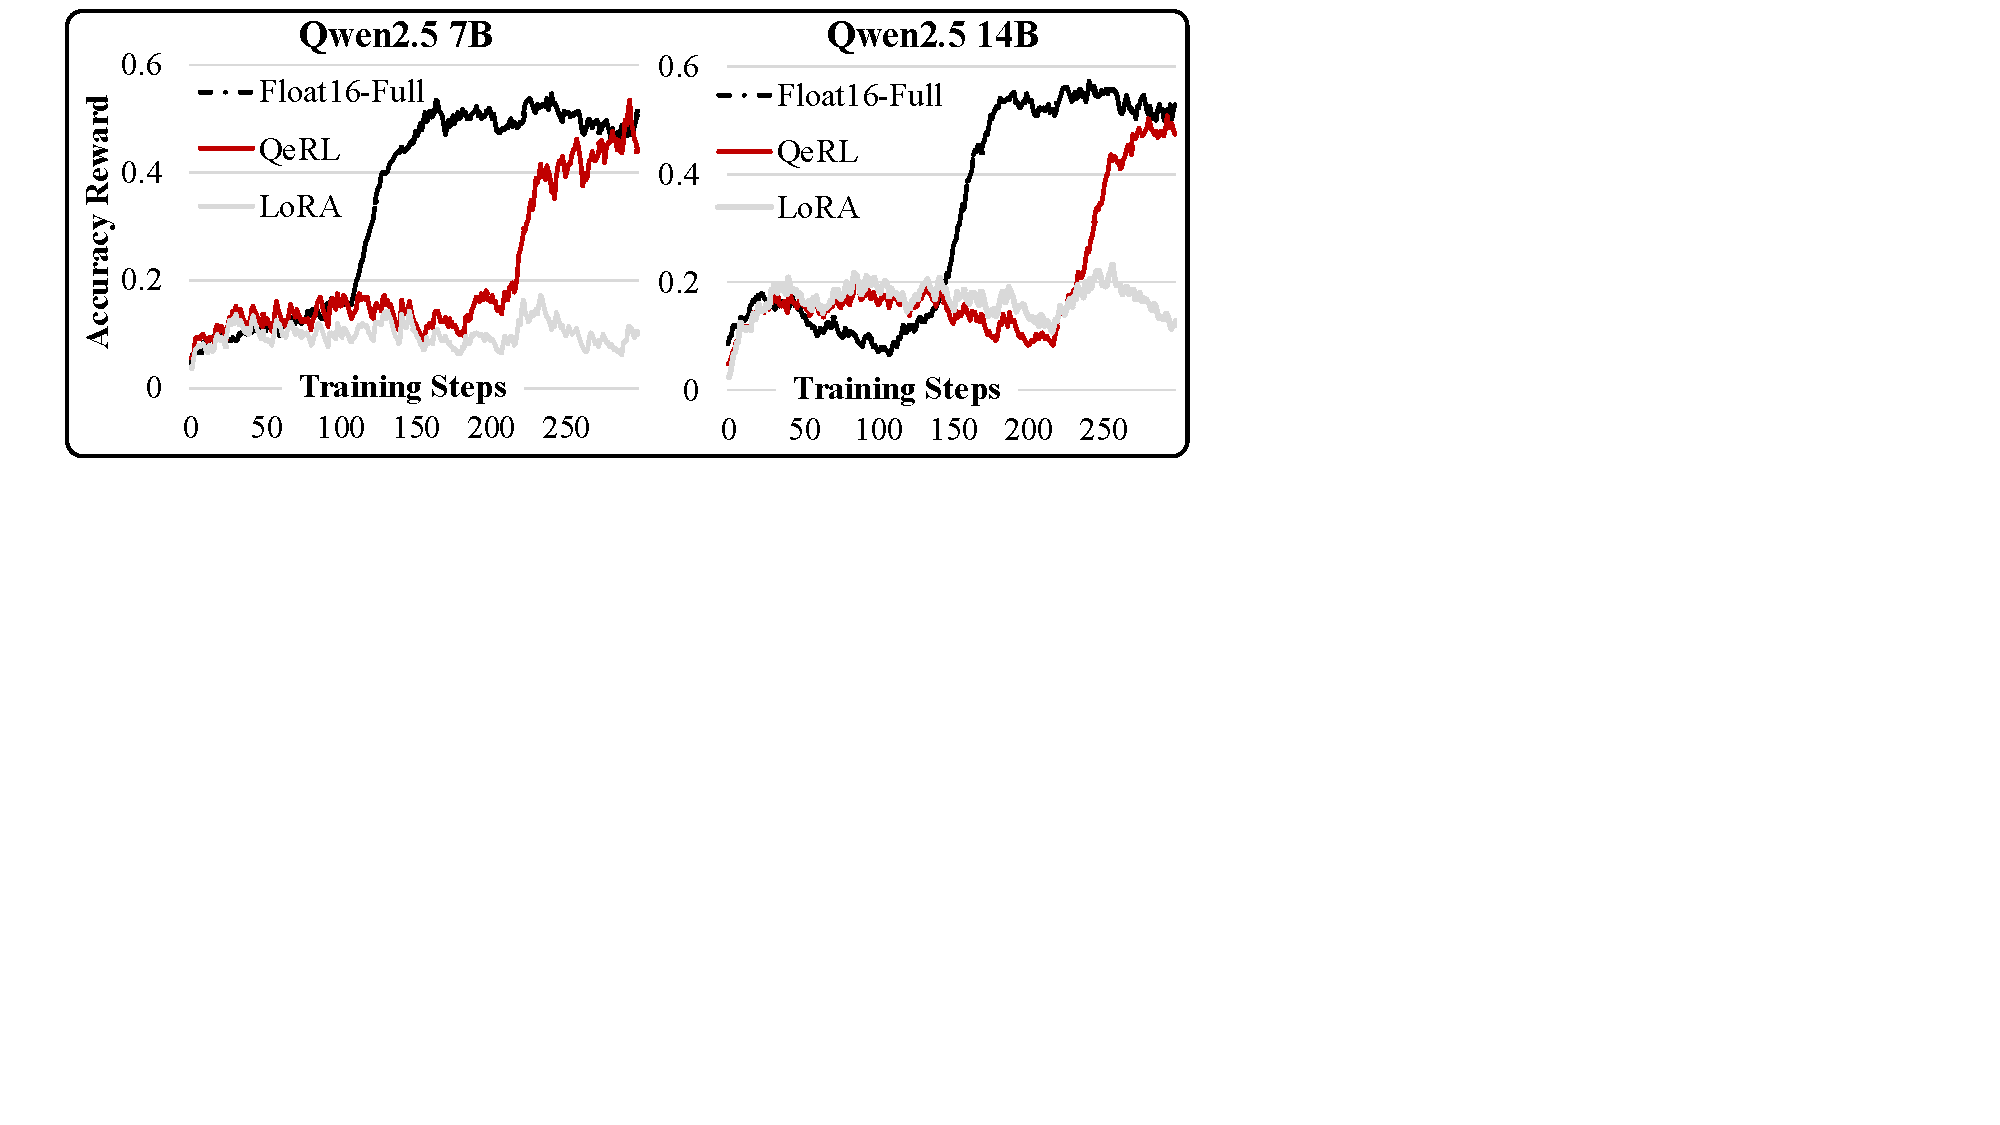
\includegraphics[width=\textwidth]{figures/fig7_1_v2.pdf}
        \vspace{-0.2in}
        \caption{Training reward of 7/14B models.}
        \label{fig:bigmath}
    \end{minipage}
    \hfill
    % 右图
    \begin{minipage}{0.49\textwidth}
        \centering
        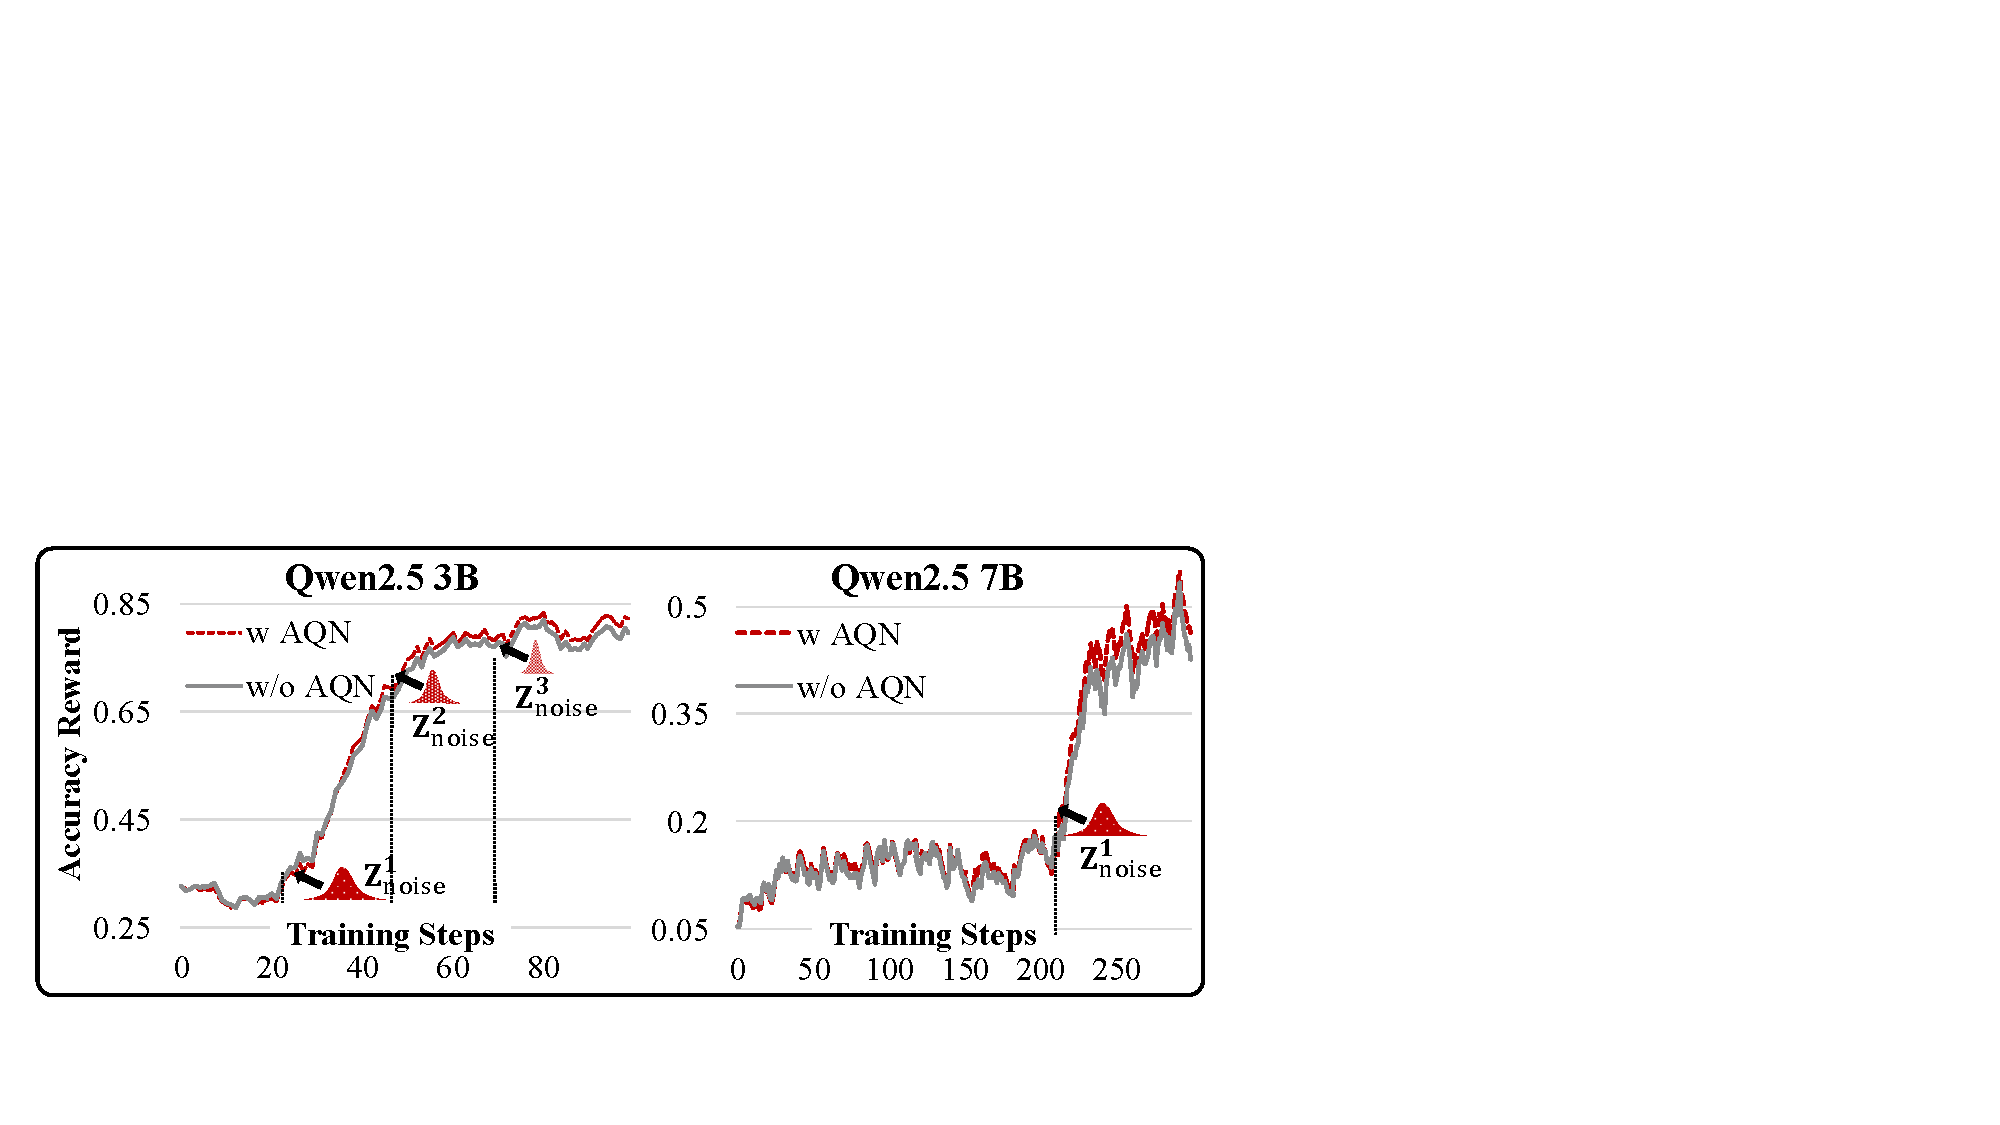
\includegraphics[width=\textwidth]{figures/fig7_2_v2.pdf}
        \vspace{-0.2in}
        \caption{Ablation of AQN on 3/7B model.}
        \label{fig:ablation_aqn}
    \end{minipage}
\vspace{-0.2in}
\end{figure}


\subsection{Experiment Results}


\textbf{Reasoning Performance}
As shown in Tab.\ref{tab:gsm8k}, we report the GSM8k training results of the 3B and 7B models using GRPO. While quantized models exhibit performance degradation compared to BF16, applying PEFT with RL to the 3B model demonstrates that NVFP4 combined with AQN achieves a performance of 83.7 from 59.4, surpassing the 76.1 achieved by 16-bit PEFT training and falling only 0.7 points below full-parameter training. Similarly, for the 7B model, our method outperforms 16-bit LoRA by 1.7 points. Furthermore, compared to QLoRA, our approach improves average accuracy by 7.6 and 5.8 points for the 3B and 7B models, respectively. Tab.\ref{tab:aime} presents the results on the BigMath dataset for the 7B, 14B, and 32B models trained with DAPO. Across all datasets, QeRL consistently matches or exceeds the performance of 16-bit models trained with LoRA. Notably, QeRL trains only about 1\% of the parameters required for full-parameter training while using just 40\%–50\% of the GPU memory of vanilla LoRA. For the 7B model, QeRL improves the average score from 25.7 (quantized) to 36.4, compared to 35.7 with vanilla LoRA. Similar trends are observed in the 14B and 32B models, where QeRL consistently outperforms vanilla LoRA across benchmarks, further supporting the conclusion that quantization enhances RL. Remarkably, on the AMC 23 dataset, the 14B model with QeRL achieves 57.5, exceeding 55.0 of full-parameter training.
% As shown in Tab.~\ref{tab:gsm8k}, we present the GSM8k training results of the 3B and 7B models with GRPO. While quantized models experience some performance loss compared to BF16, applying PEFT with RL to the 3B model demonstrates that NVFP4 combined with AQN achieves a performance of 83.7, surpassing the 76.1 of 16-bit PEFT training and falling only 0.7 points short of full-parameter training. Similarly, for the 7B model, our method outperforms 16-bit LoRA training by 1.7 points, reaching performance closer to full-parameter training. Furthermore, compared to traditional QLoRA, our approach improves average accuracy by 7.6 and 5.8 points for the 3B and 7B models, respectively. Tab.~\ref{tab:aime} presents the evaluation results of the 7B, 14B, and 32B models trained on the BigMath dataset with DAPO. Across all datasets, QeRL consistently achieves results equal to or better than those of 16-bit models trained with LoRA. This is particularly notable since QeRL trains only about 1\% of the parameters required for full-parameter training while using just 40\%–50\% of the GPU memory of vanilla LoRA. For the 7B model, QeRL improves the average score from 25.7 (quantized) to 36.4, compared to 35.7 achieved by vanilla LoRA. Similar trends are observed in the 14B and 32B models, where QeRL outperforms vanilla LoRA on most benchmarks, supporting our conclusion that quantization enhances RL. Notably, on the AMC 23 dataset, the 14B model trained with QeRL achieves a score of 57.5, even exceeding the 55.0 obtained from full-parameter training.

% \begin{wrapfigure}{h}{0.45\textwidth}
% \vspace{-0.2in}
%     \centering
%     \includegraphics[width=0.45\textwidth]{figures/rank_ab.pdf} 
%     \vspace{-0.25in}
%     \caption{
%     Ablation of LoRA rank.
%     }
%     \label{fig:ab_lora}
% \vspace{-0.1in}
% \end{wrapfigure}
\begin{figure}[!t]
\vspace{-0.2in}
    \centering
    \scalebox{1}{ % 缩放开始
    % 左图
    \begin{minipage}{0.45\textwidth}
        \centering
        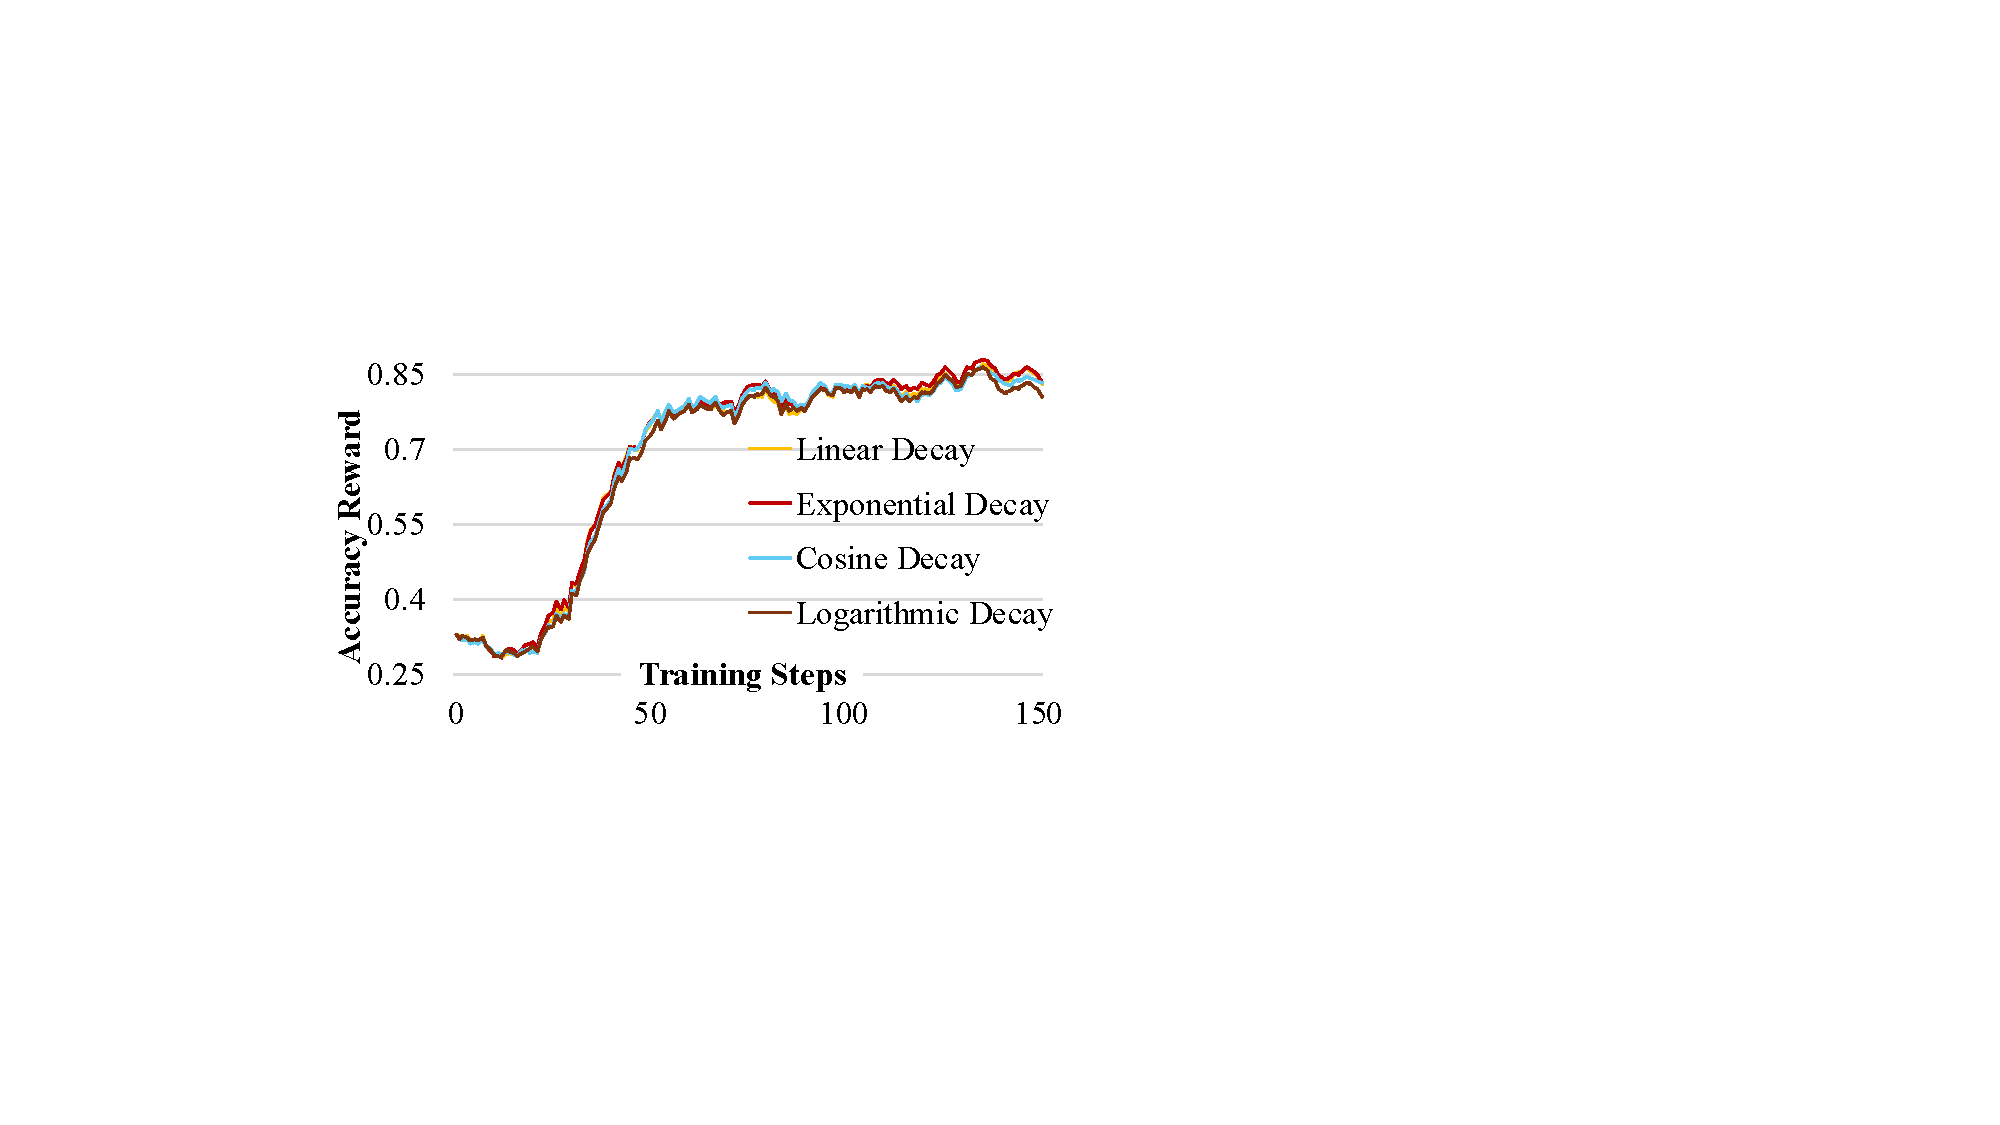
\includegraphics[width=\textwidth]{figures/scheduler_ablation_v2.pdf}
        \vspace{-0.2in}
        \caption{Comparison of noise schedulers.}
        \label{fig:noise_scheduler}
    \end{minipage}
    % 右图
        \hspace{0.1in}
    \begin{minipage}{0.49\textwidth}
        \centering
        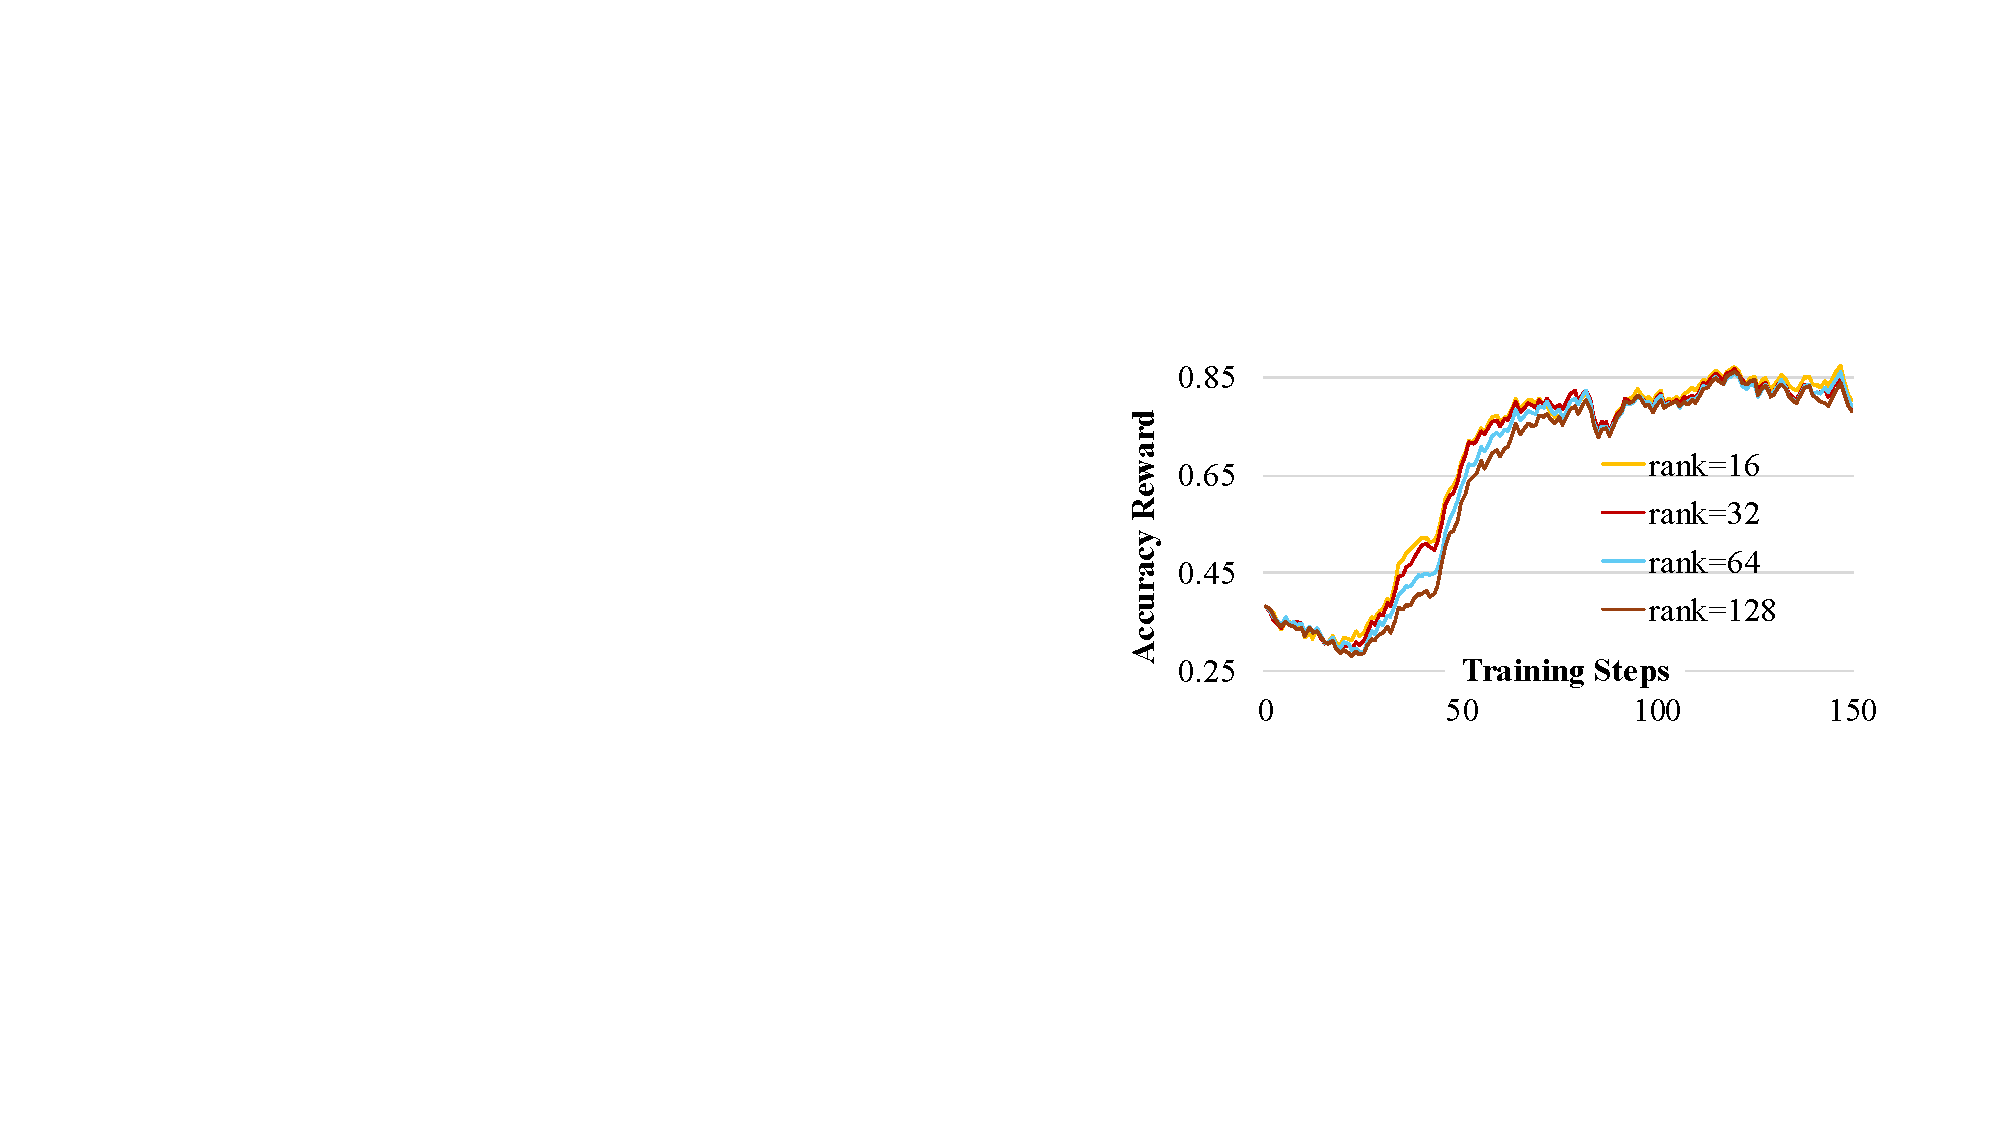
\includegraphics[width=\textwidth]{figures/rank_ablation_v2.pdf}
        \vspace{-0.2in}
        \caption{Ablation of LoRA rank.}
        \label{fig:ab_lora}
    \end{minipage}
    } % 缩放结束
\vspace{-0.2in}
\end{figure}

\textbf{Reward Visualization} 
In Sec.\ref{sec:4.2}, we compare the accuracy rewards of quantized LoRA, vanilla LoRA, and full-parameter training under GRPO and DAPO. Fig.\ref{fig:bigmath} presents the accuracy reward curves for the 7B and 14B models on the challenging BigMath dataset. Notably, QeRL achieves a rapid reward increase within 200 steps, while vanilla LoRA requires over 500 steps (Appendix~\ref{ap:more_reward}) to show improvement. This finding highlights that the inherent noise introduced by quantized LLMs enhances exploration in RL, enabling faster reward growth and higher reward targets.

\textbf{Noise Decay Schedule} \label{sec:ablation_decay}
Fig.\ref{fig:noise_scheduler} compares the performance of different noise decay functions for the 3B model: linear, exponential, cosine, and logarithmic decay. While their performance differences are negligible in the early training stages, exponential decay achieves more stable improvements later by reducing noise to lower levels. The corresponding decay curves are provided in Appendix~\ref{ap:noise}.

% \begin{figure*}[ht]
% \begin{center}
% \includegraphics[width=\linewidth]{figures/Framework.pdf}
% \end{center}
% \caption{}
% \label{fig:pipeline}
% \end{figure*}

\begin{table}[!t]
\vspace{-0.1in}
\centering
%\resizebox{\columnwidth}{!}{
\begin{tabular}{ccccccc}
\toprule
\multirow{2}{*}{\textbf{Model}}&\multirow{2}{*}{\textbf{Method}} & \multirow{2}{*}{\textbf{W\#}} & \multirow{2}{*}{\textbf{Model Size}} &\multicolumn{3}{c}{\textbf{Training Speedup} (Batch Size)}\\ 
\cmidrule(lr){5-7}
&&&&2&4&8 \\ 
\midrule
\multirow{3}{*}{\makecell{Qwen2.5-7B-Instruct}} 
%&LoRA&BF16  & 15.2 GB& $\times$1 & $\times$1 & $\times$1 \\  
&LoRA&BF16  & 15.2 GB& - & - & - \\  
&QLoRA&NF4  & 5.7 GB &$\textcolor{hangrey}{\times0.8\downarrow}$&$\textcolor{hangrey}{\times0.8 \downarrow}$&$\textcolor{hangrey}{\times0.7 \downarrow}$  \\
%\cdashline{2-7}
&\textbf{QeRL}&\textbf{NVFP4}  & {5.9 GB} & $\textcolor{hanred}{\times\mathbf{1.5}\uparrow}$&$\textcolor{hanred}{\times\mathbf{1.4}\uparrow}$&$\textcolor{hanred}{\times\mathbf{1.2}\uparrow}$ \\ 
\midrule \midrule 
\multirow{3}{*}{\makecell{Qwen2.5-14B-Instruct}} & LoRA&BF16  & 29.6 GB & - & - & - \\ 
&QLoRA&NF4  & 10.2 GB &$\textcolor{hangrey}{\times0.9\downarrow}$&$\textcolor{hangrey}{\times0.7 \downarrow}$&$\textcolor{hangrey}{\times0.7 \downarrow}$   \\
%\cdashline{2-7}
&\textbf{QeRL}&\textbf{NVFP4}  & {10.6 GB} & $\textcolor{hanred}{\times\mathbf{1.4}\uparrow}$&$\textcolor{hanred}{\times\mathbf{1.2}\uparrow}$&$\textcolor{hanred}{\times\mathbf{1.2}\uparrow}$ \\ 
% \midrule
% \multirow{6}{*}{\makecell{14B}} 
% &LoRA&BF16  & 29.6& 1 & 65.4 &&470.9&& \\ 
% &QLoRA&NF4  &10.1& 1 & 55.9&$\textcolor{hangrey}{\times0.9\downarrow}$&302.8&$\textcolor{hangrey}{\times0.6\downarrow}$&$\textcolor{hangrey}{\times0.7\downarrow}$   \\
% \cdashline{2-10}
% &\textbf{QeRL}&\textbf{NVFP4}  & 10.6& 1  & \textbf{98.3}&$\textcolor{hanred}{\times\mathbf{1.5}\uparrow}$ &\textbf{979.6}&$\textcolor{hanred}{\times\mathbf{2.1}\uparrow}$ \\ 
% \cline{2-10}
% &LoRA&BF16  &29.6& 16 &737.2&&6194.8&& \\ 
% &QLoRA&NF4  &10.1& 16&560.3&$\textcolor{hangrey}{\times0.8\downarrow}$&4398.3&$\textcolor{hangrey}{\times0.7\downarrow}$&$\textcolor{hangrey}{\times0.6\downarrow}$   \\ 
% \cdashline{2-10}
% &\textbf{QeRL}&\textbf{NVFP4}   &  10.6& 16 &\textbf{1091.1}&$\textcolor{hanred}{\times\mathbf{1.5}\uparrow}$&\textbf{14417.9}&$\textcolor{hanred}{\times\mathbf{2.3}\uparrow}$ \\ 
\bottomrule
\end{tabular}
%}
\caption{Memory Saving and Speedup of 7B and 14B models. We report the end-to-end speedup in the GRPO process of each training step. Each input has a length of 256 tokens, and each max completion length is 2048. More results of other models are shown in Appendix~\ref{ap:efficient}.} \label{tab:efficiency_7b_and_14b}
\end{table}


% \subsection{Ablation Results}

\textbf{Ablation of AQN}
Using default quantized noise throughout the training limits the exploration in RL. To address this, we propose the AQN. As shown in Fig.\ref{fig:ablation_aqn}, when we start with the default quantized noise and periodically inject additional noise in later stages, the reward curve grows more steadily. Notably, when the reward approaches convergence, AQN effectively expands the model's exploration space, enabling further improvements in reward.

\textbf{Ablation of LoRA Rank}
Fig.\ref{fig:ab_lora} compares the reward curves of the 3B model during QeRL with different LoRA ranks. Specifically, ranks of 16, 32, 64, and 128 exhibit similar trends and reward growth rates, with rank 16 converging slightly faster, making it a more economical choice. 


\begin{figure*}[!t]
\vspace{-0.1in}
\begin{center}
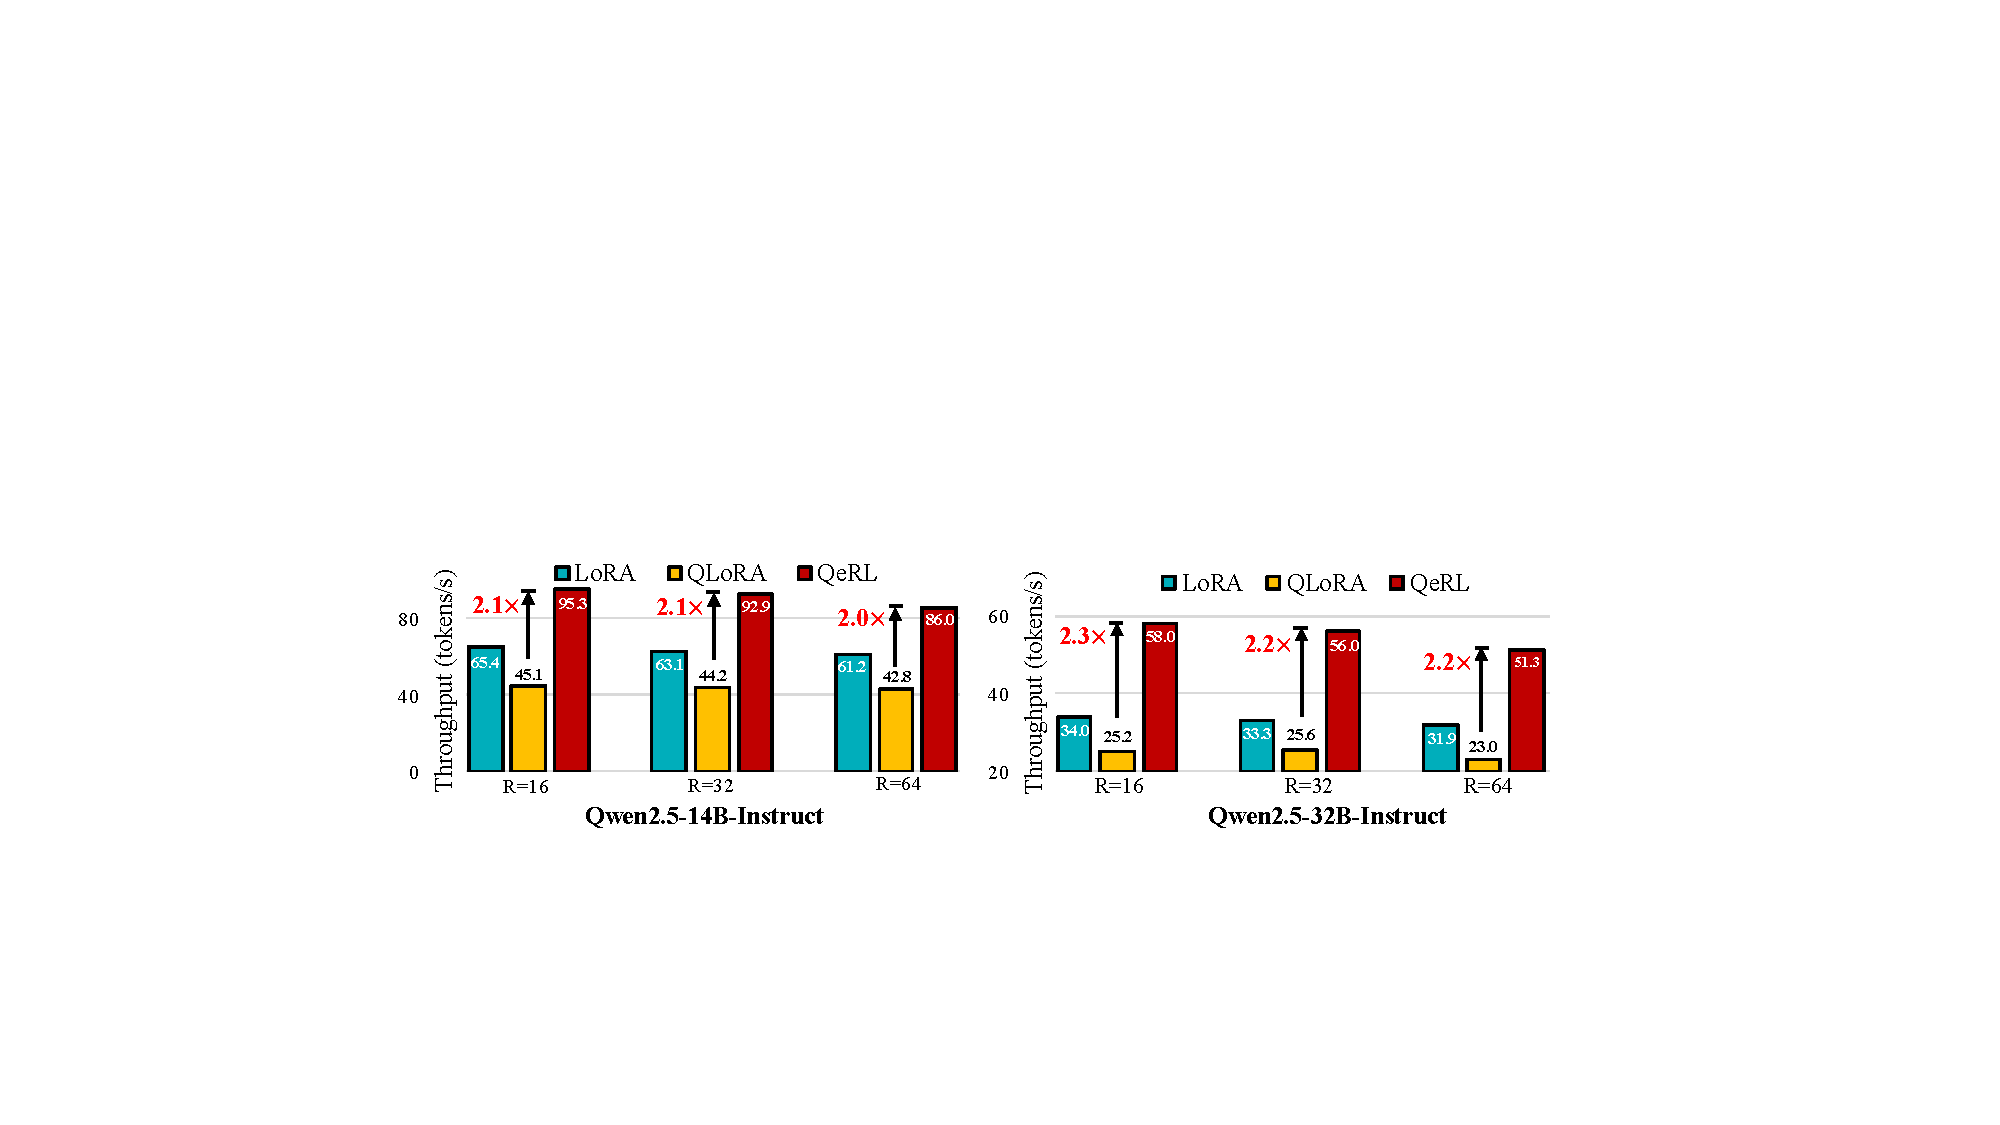
\includegraphics[width=1\linewidth]{figures/rank_speed_v2.pdf}
\end{center}
\vspace{-0.1in}
\caption{Rollout throughput of 14/32B model. The setting is aligned with Tab.~\ref{tab:efficiency_14b} (batch is 1).}
\label{fig:rollout_throughput}
\vspace{-0.1in}
\end{figure*}

\subsection{Memory Saving and Speedup}
Tab.\ref{tab:efficiency_7b_and_14b} compares the quantized model sizes and end-to-end RL training speedup of these PEFT methods, with all experiments conducted on a single NVIDIA H100-80GB GPU~\citep{noauthor_nvidia_nodate}. For 7B and 14B models, both QLoRA (NF4) and QeRL (NVFP4, supported by the Marlin kernel~\citep{frantar2024marlin}) significantly reduce memory usage, shrinking the model sizes to 25\%–30\% of their 16-bit counterparts. Due to the limitations of NF4 generation speed~\citep{egashira2024exploiting}, QLoRA slows to 0.7$\times$–0.8$\times$ across different batch sizes. In contrast, QeRL achieves 1.2$\times$–1.5$\times$ training speedups over vanilla LoRA, benefiting from the generation speed of long reasoning sequences. This efficiency is particularly evident in RL, where the computational demands of long-horizon rollouts emphasize QeRL's advantage. Notably, our speedup measurements are based on the average speed during the first 30 steps, where the output token length is relatively short. In later stages of training, as the model generates longer outputs, the speed advantage of QeRL becomes even more pronounced. Its dual benefits in memory efficiency and training speed make QeRL highly effective for end-to-end RL workflows, especially in scenarios requiring extensive rollouts. Fig.\ref{fig:rollout_throughput} shows rollout performance across various LoRA ranks, with QeRL achieving over 2$\times$ speedups on 14B and 32B models. More efficiency comparisons for other models and settings are in Appendix~\ref{ap:efficient}. 